%\RequirePackage{fix-cm}
\documentclass{ntuthesis}

\usepackage{times}
\usepackage{verbatim}
\usepackage{color}
\usepackage{url}
\usepackage{graphicx}
\usepackage{amsmath}
\usepackage{array}
\usepackage{wallpaper}

% Using the tex-text mapping for ligatures etc.
\defaultfontfeatures{Mapping=tex-text}

% Set the default fonts
\setmainfont{times.ttf}
\setCJKmainfont{kaiu.ttf}

% Watermark
\CenterWallPaper{0.174}{watermark.pdf} 
\setlength{\wpXoffset}{6.1725cm}
\setlength{\wpYoffset}{10.5225cm}   

\newgeometry{top=3cm,left=3cm,bottom=2cm,right=3cm}

% Your information goes here
% author: Tz-Huan Huang [http://www.csie.ntu.edu.tw/~tzhuan]

% ----------------------------------------------------------------------------
% "THE CHOCOLATE-WARE LICENSE":
% Tz-Huan Huang wrote this file. As long as you retain this notice you
% can do whatever you want with this stuff. If we meet some day, and you think
% this stuff is worth it, you can buy me a chocolate in return Tz-Huan Huang
% ----------------------------------------------------------------------------

% Syntax: \var{English}{Chinese}
\university{National Taiwan University}{國立臺灣大學}
\collage{College of Electrical Engineering and Computer Science}{電機資訊學院}
\institute{Department of Computer Science and Information Engineering}{資訊工程學系}
\title{English thesis name here}{中文論文名字}
\author{Author's english name}{作者中文名字}
\studentid{R029220xx}
\advisor{my boss, Ph.D.}{某某某 博士}
\defenseyear{2015}{104}
\defensemonth{July}{7}
\defenseday{21}


\begin{document}

\frontmatter 
\makecover 
\makecertification

\begin{acknowledgementszh}

謝啦各位

\end{acknowledgementszh}

\begin{acknowledgementsen}

Thanks!

\end{acknowledgementsen}

\begin{abstractzh}

在實際的應用上,...,此方法可以套用在圖像處理器上進行平行運算以達到更高的加速。
{\bf 關鍵字:} 大規模物件偵測、稀疏編碼

\end{abstractzh}

\begin{abstracten}
	
For practical applications, ... This misuse results in huge accuracy loss when a large speedup is required. ...
{\bf Keyword:} Scalable object detection, Sparse coding

\end{abstracten}



\tableofcontents
\listoffigures
\listoftables

\mainmatter

% You can organize your own chapter 
\chapter{Introduction}
\label{c:intro}

In object detection, many works based on part-based model such as the Deformable Part Model (DPM) \cite{voc-release5}.

To tackle the problem, we proposed Regularized Sparse Coding which is optimized for filter functionality\protect\footnotemark[1].

\footnotetext[1]{In this work we call the ability of filter to produce accurate score map in object detection as \textit{filter functionality}.}

\begin{itemize}
  \item We propose Regularized Sparse Coding to reconstruct filter functionality which sparse coding cannot reconstruct successfully.
  \item We conduct experiments on several large datasets with up to 200 classes to prove scalability of our method. 
  \item We achieve 16 times speedup using only 1.25\% memory with less than 0.04 mAP drop compared to the original Deformable Part Model.
\end{itemize}
\chapter{Related Work}
\label{c:relate}

In general, object detection can be reduced to proposal extraction and object classification. So, the computational complexity of object detection could be $\mathcal{O}(LC)$, where L is the number of proposals and C is the number of classes. These two stages and the impacts on scalability are discussed separately in this section.

\section{Proposal Extraction}

From the famous cascade method \cite{viola2001rapid}, many works ...

\section{Object Classification}

With the exception of few object detection frameworks \cite{chen2013efficient, murphy2006object} ...
\chapter{Technical Details}
\label{c:tech}

In this section we describe a framework based on the Deformable Part Model (DPM) ...

\section{Sparse Coding}

\begin{equation} \label{eqOMP}
  \begin{aligned}
    & \min_{\alpha_{ij}, D_j}\sum
    _{i=1}^N&&\begin{Vmatrix}X_i-\sum_{j=1}^K\alpha_{ij}D_j\end{Vmatrix}_2^2\\
    & \text{subject to} && \left \| \alpha_i \right \|_0 \leq 
    \epsilon, \forall i=1,...,N\\
    &&& \left \|D_j \right \|_2 = 1, \forall j=1,...,K
  \end{aligned}
\end{equation}
%

In Equation \ref{eqOMP} ...

\section{Regularized Sparse Coding} \label{secRSC}

The previous section has shown the capability of sparse coding, but here we provide some observations to help revise sparse coding into our method, which is called Regularized Sparse Coding. ...

\chapter{Experiment Results} \label{secEXP}
\section{Datasets and Implementation}

\textbf{Pascal Visual Object Classes Challenge 2012 (VOC2012) \cite{pascal-voc-2012}.} This famous object detection benchmark consists of 20 classes. We use this dataset to show our work's capability in reducing computing time. Training set and validation set are used to train models while the test set is used to evaluate performance. Notice that this dataset only has a relative small number of classes but the experiment result proves that we can perform well on it. In Figure. \ref{figFeatureUsage}...

\begin{figure}
\centering
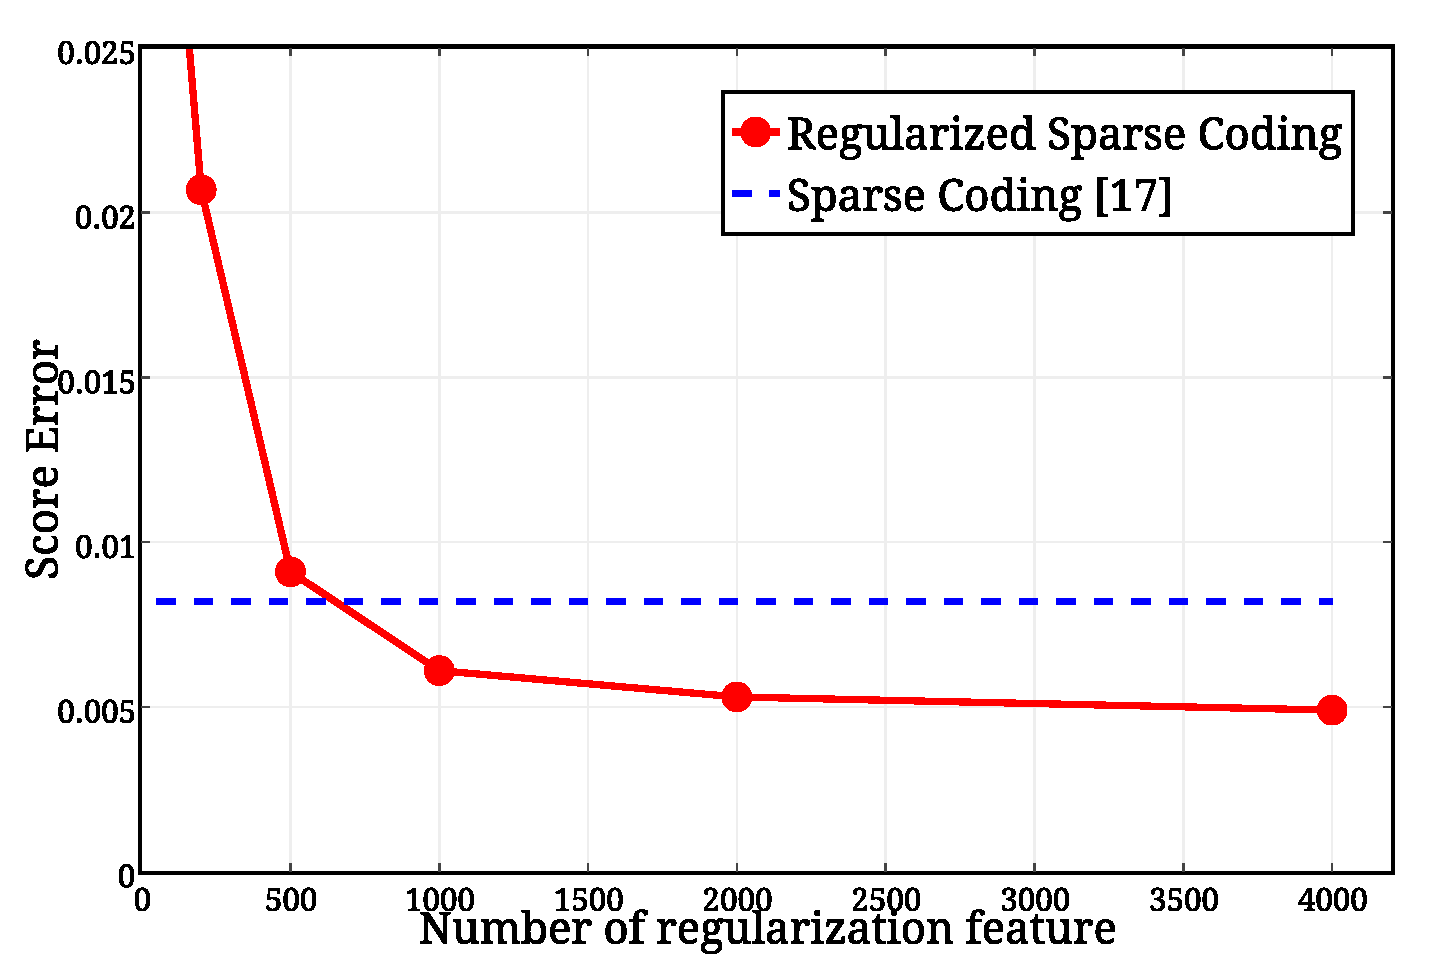
\includegraphics[width=0.48\textwidth]{featureUsage}
\caption{Effect of the number of regularization features used in Regularized Sparse Coding\protect\footnotemark[3]. As the solid line illustrates, the score error drops with more features involved. The dotted line is the original sparse coding method. Although sparse coding also has low score error, small difference of score error between the two method will result in a huge performance difference (mAP) in later experiments.}
\label{figFeatureUsage}
\end{figure}

\section{Performance Analysis}

\section{Scalability}

To compare sparse coding with our method, we conduct experiments on ILSVRC2013 ...


\chapter{Conclusion}
\label{c:conc}

In this work we proposed a method called ..., to provide speedup without accuracy loss and huge memory usage.


\appendix

\backmatter

\addcontentsline{toc}{chapter}{\bibname}
\bibliographystyle{abbrv}

% Your bibliography goes here
\bibliography{thesis}

\end{document}
